%% LyX 2.0.1 created this file.  For more info, see http://www.lyx.org/.
%% Do not edit unless you really know what you are doing.
\documentclass[english,conference]{IEEEtran}
\usepackage[T1]{fontenc}
\usepackage[latin9]{inputenc}
\usepackage{color}
\usepackage{array}
\usepackage{float}
\usepackage{amsmath}
\usepackage{amssymb}
\usepackage{graphicx}
%\usepackage{esint}
%\usepackage{subscript}

\makeatletter

%%%%%%%%%%%%%%%%%%%%%%%%%%%%%% LyX specific LaTeX commands.
%% Because html converters don't know tabularnewline
\providecommand{\tabularnewline}{\\}
%% A simple dot to overcome graphicx limitations
\newcommand{\lyxdot}{.}

\floatstyle{ruled}
\newfloat{algorithm}{tbp}{loa}
\providecommand{\algorithmname}{Algorithm}
\floatname{algorithm}{\protect\algorithmname}

%%%%%%%%%%%%%%%%%%%%%%%%%%%%%% Textclass specific LaTeX commands.
\newenvironment{lyxcode}
{\par\begin{list}{}{
\setlength{\rightmargin}{\leftmargin}
\setlength{\listparindent}{0pt}% needed for AMS classes
\raggedright
\setlength{\itemsep}{0pt}
\setlength{\parsep}{0pt}
\normalfont\ttfamily}%
 \item[]}
{\end{list}}

%%%%%%%%%%%%%%%%%%%%%%%%%%%%%% User specified LaTeX commands.

\usepackage{cite}\@ifundefined{definecolor}
 {\usepackage{color}}{}
\usepackage{amsfonts}\usepackage{mathtools}\usepackage{multirow}\usepackage{subfigure}\usepackage{tikz}\usepackage{pgf}\usepackage{pgfplots}\DeclareGraphicsExtensions{.pdf,.png,.jpg,.eps}
%\pgfplotstableread{Experiments/noexp.dat}\noexp

\makeatother

\usepackage{babel}
\begin{document}

\title{Stencil processing on single-core, multicore, and GPU architectures}


\author{\IEEEauthorblockN{Sami Wilf, Dinesh Agarwal, and Abinashi Dhungel}
\IEEEauthorblockA{ Georgia State University\\
 Department of Computer Science\\
 Atlanta, Georgia 30303\\
 } }
\maketitle
\begin{abstract}
This work explores multi-core parallelization and introduces a pair-symmetric
algorithm for stencil codes. Specifically, we use the bilateral filter
as our example stencil code for which we implemented both our pair-symmetric
algorithm and the standard naive stencil code algorithm. The bilateral
filter is a non-iterative image processing filter used to smooth images
without blurring pictorial edges. While it is an embarrassingly parallel
algorithm, it is still extremely compute intensive. In this paper,
we focus on both reducing and mitigating the effects of this computational
intensity and provide methods for improving the performance of bilateral
filtering, which consist of the elimination of redundant calculations
using our pair-symmetric algorithm implemented in Nvidia\textquoteright{}s
Compute Unified Device Architecture (\textquotedblleft{}CUDA\textquotedblright{}),
the use of low level single instruction, multiple data (\textquotedblleft{}SIMD\textquotedblright{})
parallelism, and the use of thread level parallelism and reduction.
We also present empirical data evidencing the performance gains we
achieved across the variety of architectures. The hardware used consists
of Nvidia GTX280, Advanced Micro-devices Devices (``AMD'') Barcelona,
AMD Shanghai, AMD Phenom, Intel Harpertown, Intel Lynnfield (Core
i7) quad core, and Intel Nehalem 32 core machines. The best speedup
achieved was a 235.5x speedup by our CUDA-based implementation of
our pair-symmetric stencil algorithm running on Nvidia's GTX280. Our
CPU multicore implementations resulted in a speedup of up to 38x using
16 cores of AMD Barcelona each with 4-stage vector pipeline, up to
23x using 8 cores for Intel Harpertown compared to a compiler optimized
code exploiting 4-stage vector unit of a core, we further demonstrate
speedup of up to 26x using 32 cores of Intel Nehalem multicore architecture.
\end{abstract}
% For peer review papers, you can put extra information on the cover
% page as needed:
% \ifCLASSOPTIONpeerreview
% \begin{center} \bfseries EDICS Category: 3-BBND \end{center}
% \fi
% For peerreview papers, this IEEEtran command inserts a page break and
% creates the second title. It will be ignored for other modes.
\IEEEpeerreviewmaketitle


\section{Introduction}

\label{sec:intro} The recent advances in parallel computing have
provided a series of avenues for achieving significant increases in
performance. However, unlike the days when applications automatically
became faster with increased clock frequency, multicore chips require
programmers and researchers to revisit their algorithm designs to
harness the power of underlying architectures. Moreover, there is
no well defined list of guidelines that can be followed for each application.
This makes it more challenging to deploy existing applications, even
fundamental ones, to a myriad of available multicore architectures.

As reported in \cite{landscapeofpc} one of the critical questions
for parallel computing community is to identify the common kernels
being used in various applications. One such kernel is the Bilateral
filter, a non-iterative image processing kernel widely used to perform
directionally dependent image smoothing. In this paper we propose
a set of optimizations and a non-naive algorithm for stencil codes.
Specifically, we introduce a pair-symmetric stencil code algorithm
which has the theoretical potential to cut processing time in half.
We also propose architecture specific optimizations, such as by exploiting
the unique capabilities of special registers available in modern multicore
architectures and the rearrangement of data access patterns as per
the computations to exploit special purpose instructions. We also
propose optimizations for stencil code processing on Nvidia's CUDA,
with such optimizations including the utilization of CUDA's implicit
synchronization capability and the maximization of single-instruction
per multiple-thread efficiency. 

we use the bilateral filter as our example stencil code\textcolor{blue}{{}
}\textcolor{black}{since it has not only been used for image processing
but also as a benchmarking kernel for various architectures\cite{Kamil2010}.
Moreover, because our optimizations are equally applicable to other
kernels such as 3D heat equation, matrix multiplication, and other
Jacobi iterations, our research will contribute to more than just
image processing applications.}

Our methods are effective over a range of multicore chips with varying
number of cores. In order to assess the effi{}cacy of our optimization
techniques, our experimental testbed includes a comprehensive set
of multicore architecture chips including the Nvidia GTX280, AMD quad-core
2376 (Shanghai), AMD quad-core 8350 (Barcelona), Intel quad-core Xeon
E5410 (Harpertown), Intel eight-core Xeon X7560 (Nehalem-EX), Intel
quad-core Core i7(Lynnfi{}eld) and AMD Phenom II six-core architectures.


\section{Bilateral Filtering Basics}

\label{sec:stencil} 
\begin{figure}[!h]
\centering 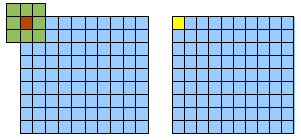
\includegraphics[width=3.2in]{filter} \caption{Example of a filter at the starting position of the image}


\label{fig:filter} 
\end{figure}


Filtering is a fundamental image processing operation that finds its
application in a variety of tasks, such as filtering out noise, edge
detection, edge highlighting, and pre-processing tasks for higher
level image processing operations such as object recognition and face
recognition, among other things. Filtering is carried out by a relatively
small window, known as the filter (``Filter'' or ``Window''),
which iterates over the source image, performing the same execution
at each step of the iteration. The elements that the Filter's covers
in a given iteration makeup the neighborhood (``Neighborhood'')
and are neighbors (``Neighbors'' or ``Neighboring Pixels'') of
the Filter's center element (``Center'' or ``Center Pixel'').
\ref{fig:filter}illustrates the starting position of the Filter as
commonly seen in standard, naive stencil algorithms; the source image
is on the left and the destination image on the right is used store
the result of the Filter's computation at the respective Center's
position.

Our work explores the bilateral filtering kernel proposed by Tomasi
and Manduchi \cite{Tomasi1998} which is used to smooth an image without
blurring its edges. A faster approximation to the original algorithm
\cite{Paris2009} extends the image to 3D space by treating the pixel
intensity as the third dimension and using a linear shift-invariant
convolution in 3D. A separable implementation \cite{Pham2005} applies
the filter kernel first to one of the image dimensions and the intermediate
result is filtered again on other dimensions. This reduces the complexity
from $O(N*(m^{d}))$ to $O(N*d)$ where $N$ is the total number of
pixels in the image and $d$ is the dimensionality of image. However,
we do not parallelize these faster methods since our interest is to
develop a parallelization method that can be applied, in general,
to any spatially invariant and inseparable stencil code.

\textcolor{black}{Bilateral filtering combines two different kernels---the
spatial kernel and the photometric kernel. With the photometric kernel,
when the Center of the Filter rests on a pixel that boarders or is
a part of a pictorial edge, }\textit{\textcolor{black}{e.g.}}\textcolor{black}{,
an outline of an object or person against a contrasting background,
the Neighbors that make up the other (contrasting) side of the edge
have an insignificant impact on the Center Pixel's corresponding output
pixel, which is stored in the destination array storing the processed
image. Furthermore, when the Center is not bordering, and is not a
part of, a pictorial edge, the Neighbors contribute equally and the
noise is filtered out. Hence, pictorial edges maintain sharpness while
noise in the pictorial regions are filtered, resulting in more appealing
images. Mathematically, the Bilateral filter can be defined in terms
of the spatial kernel and photometric kernel as follows\cite{Tomasi1998}:}\\


Spatial kernel: 
\begin{equation}
h(x)=k_{d}^{-1}(x)\int_{-\infty}^{\infty}\int_{-\infty}^{\infty}f(\xi)c(\xi,x)d\xi\label{spatial}
\end{equation}
 
\begin{equation}
k_{d}(x)=\int_{-\infty}^{\infty}\int_{-\infty}^{\infty}c(\xi,x)d\xi
\end{equation}
 Photometric kernel: 
\begin{equation}
h(x)=k_{r}^{-1}(x)\int_{-\infty}^{\infty}\int_{-\infty}^{\infty}f(\xi)s(f(\xi),f(x))d\xi\label{photometric}
\end{equation}
 
\begin{equation}
k_{r}(x)=\int_{-\infty}^{\infty}\int_{-\infty}^{\infty}s(f(\xi),f(x))d\xi
\end{equation}


The combined kernel, which is the bilateral filter, is the product
of spatial kernel and photometric kernel and is described as: 
\begin{equation}
h(x)=k^{-1}(x)\int_{-\infty}^{\infty}\int_{-\infty}^{\infty}f(\xi)c(\xi,x)s(f(\xi),f(x))d\xi\label{combined}
\end{equation}
 
\begin{equation}
k^{-1}(x)=\int_{-\infty}^{\infty}\int_{-\infty}^{\infty}c(\xi,x)s(f(\xi),f(x))d\xi
\end{equation}


Function $c(\xi,x)$ measures the $geometric$ $closeness$ between
neighborhood Center $x$ and a Neighbor $\xi$. Function $s(f(\xi),f(x))$
measures the $photometric$ $similarity$ (similarity in pixel intensity)
between the same. The influence of a Neighbor on the Filter's output
computation for a Center Pixel is calculated as a product of spatial
kernel and the photometric kernel. Thus, Neighbors with similar photometric
properties influence the Center Pixel more than those with less similar
photometric properties. This results in edge-preserved image smoothing,
which is the purpose of the bilateral filter. It should be noted,
however, that the foregoing equations are mathematical representations
for filtering of infinite-precision images. As infinite-precision
is a concept more pertinent to the analog domain and does not exist
in the digital domain, each double integral in equations 1-6 must
be understood as the summation of a finite set of calculations, \textit{i.e.,}
one calculation per Neighbor and one set of calculations per Center
Pixel, or put another way, one set of calculations per Filter iteration.
A formal expression is given below:

\begin{equation}
filtered\: pixil=\frac{\substack{N\\
\sum\\
i=1
}
x_{i}\cdot c(\xi,x)\cdot s(f(\xi),f(x))d\xi}{\substack{N\\
\sum\\
i=1
}
c(\xi,x)\cdot s(f(\xi),f(x))d\xi}
\end{equation}


In addition to restating the bilateral filter's mathematical model
in terms of a finite summation, Equation 7 reveals that data dependency
exists in the bilateral filter. Specifically, Equation 7 shows that
before the filtered pixel can be calculated by dividing the numerator
by the denominator, both the summation in the numerator and summation
in the denominator must first be calculated. Consequently, the bilateral
filter has two data dependencies. As explained later in this paper,
the pair-symmetric algorithm significantly increases the memory consumption
in order to manage data dependencies but pays off by cutting in half
the total number of executions.

\textcolor{black}{Another observation taken into account is that the
values of equation (\ref{spatial}) for the Neighborhood can be computed
in advance as the values depend on a simple Gaussian probability distribution
function. However, the values of equation (\ref{photometric}) and
consequently of equation (\ref{combined}) cannot be known }\textit{\textcolor{black}{a
priori}}\textcolor{black}{{} as they depend on the similarity of signals
between the Center Pixel and the Neighborhood. Moreover, as the size
of the Window increases, which only happens by choice of the user
as the size is user defined, the number of computations per pixel
grows at a rate of $O(FilterWindowWidth^{2})$ where }\textit{\textcolor{black}{FilterWindowWidth}}\textcolor{black}{{}
is the diameter of the Window. By reason of the foregoing, the bulk
of the time spent in processing an imagine using the bilateral filter
is in the arithmetic-intensive computations, because the number of
writes to the destination image is constant as the rate of growth
of Center-Neighbor computations with respect to the Window size increases.}


\section{Stencil Processing}


\subsection{A Naive Approach to Stencil Processing}

\begin{figure}
\centering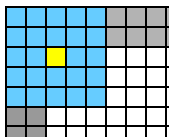
\includegraphics[scale=0.35]{/Users/Sami/programming/ALGORITHM_1/bilat/the1}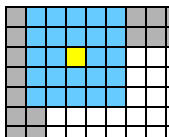
\includegraphics[clip,scale=0.35]{/Users/Sami/programming/ALGORITHM_1/bilat/the202}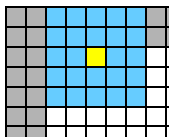
\includegraphics[scale=0.35]{/Users/Sami/programming/ALGORITHM_1/bilat/the2}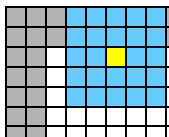
\includegraphics[scale=0.35]{/Users/Sami/programming/ALGORITHM_1/bilat/the3}

\caption{Example of a naive bilateral filter iterations}
\end{figure}


The naive stencil algorithm is the standard model that is predominantly
used. This is evidenced by the fact that all of the authors of papers
cited herein either overlook or were unable to find improvements to
the naive algorithm itself. Those authors went straight to hardware
dependent implementations and expended their resources on achieving
performance gains that did not match the effort taken. Here, we address
a root problems of the standard naive algorithm by creating a new
algorithm, and then we also develop hardware dependent improvements
for greater speedup. Below is the pseudo-code for the standard naive
stencil kernel.
\begin{algorithm}[!h]
\caption{\label{alg:Example-Algorithm-float}Naive Stencil Kernel Algorithm}

\begin{lyxcode}
for~(each~element~\textit{e}\textsubscript{i,j}~in~source~image~\textit{\footnotesize s})\{~\\
\textit{~Center\textsubscript{i,j}}~=~\textit{e}\textsubscript{i,j}~\\
~for~(each~data~dependency\textit{~n})~\\
~~\textit{set~register~X\textsubscript{n}}to~0~\\
~\textit{/{*}Complete~dependency~computations{*}/}~\\
~Begin:~\\
~for(int~\textit{k~from}~\textit{-filter\_hw~to}~\textit{filter\_hw})~\\
~for(int~\textit{l}~from~\textit{-filter\_hw}~to~\textit{filter\_hw})\{~\\
~~for~(~each~data~dependency~\textit{n})~\\
~~\textit{X\textsubscript{n}}+=Funct\textit{\textsubscript{n}}(\textit{\footnotesize s}{[}\textit{Center\textsubscript{i,j}}{]},\textit{\footnotesize s}{[}\textit{Neighbor\textsubscript{i+k,j+l}}{]})~\\
~\}~\\
~End~\\
~\textit{/{*}Dependency~computations~completed{*}/}~\\
\textit{~/{*}obtain~output~from~dependency~data{*}/}~\\
~outImg{[}\textit{Center\textsubscript{i,j}}{]}=computeOutputPixel(\textit{\&X})~\\
\}

\end{lyxcode}
\end{algorithm}



\subsection{Pair-symmetric Stencil Processing}
\begin{itemize}
\item \textit{\textcolor{black}{Advantages: Reduces by half the amount of
Center-Neighbor computations, and can theoretically cut processing
time in half.}}
\item \textit{\textcolor{black}{Disadvantages: RequIres more memory which
increases with the amount of dependencies.}}
\item \textit{\textcolor{black}{Implementation obstacles: race-conditions}}
\end{itemize}
Our pair-symmetric stencil algorithm is premised on the fact that
each pixel assumes the role of both a Center Pixel and a Neighboring
Pixel and that stencil codes are symmetric with respect to Center-Neighbor
paired computations. For example, in the bilateral filter, $c(\xi,x)$
returns the same value as $c(x,\xi)$ and $s(f(\xi),f(x))$ returns
the same value as $s(f(x),f(\xi))$. It then follows that the naive
stencil algorithm dictated in Algorithm 1 above performs twice as
many calculations as are necessary.

Our pair-symmetric algorithm eliminates this redundancy that is inherent
in the naive stencil code algorithm. Instead of reading from all Neighbors,
our pair-symmetric algorithm reads from only half of the Neighbors.
The result of each Center-Neighbor paired computation is then added
to the \textit{X\textsubscript{n}}register, which eventually obtains
the result of data dependency \textit{n}. This is trivial as the naive
stencil algorithm already does this. What our algorithm does that
is unique is that the result of each Center-Neighbor pair computation
is also added to and stored in the Neighbor's position in a temporary
array (``Map'') that is used for storing the results of a data dependency.
So, there are \textit{N} Maps for \textit{N} number of dependencies.
After the data dependency conditions are met, the function that returns
the output data from the dependencies iterates over the Maps. As applied
to the bilateral filter, the data dependency lies in calculating each
pixel's numerator and denominator that is used to derive the pixel's
output result. After the numerators and denominators are derived,
a function iterates and devised the corresponding elements of the
two arrays to return the output. The pseudocode is given below:
\begin{algorithm}[h]
\noindent \caption{\label{alg:Example-Algorithm-float-1}Pair-symmetric Stencil Algorithm}

\begin{lyxcode}
\noindent \textit{for~(each~element~e\textsubscript{i,j}~in~source~image~}\textit{\footnotesize s}\textit{)\{}~\\
\textit{~~Center\textsubscript{i,j}~=~e\textsubscript{i,j}}~\\
\textit{~~for~(each~data~dependency~n)}~\\
\textit{~~~~float~X\textsubscript{n}=~0}~\\
\textit{~~for(~k~from~0~to~filter\_hw)}~\\
\textit{~~for(~l~from~0~to~filter\_hw)}~\\
\textit{~~for~(~each~data~dependency~n)~\{}~\\
\textit{~~~~temp~=~}

\textit{~~~~funct\textsubscript{n}(}\textit{\footnotesize s}\textit{{[}Center\textsubscript{i,j}{]},}\textit{\footnotesize s}\textit{{[}Neighbor\textsubscript{i+k,j+l}{]})}~\\
\textit{~~~~X\textsubscript{n}+=~temp}~\\
\textit{~~~~dependencyArray\textsubscript{n}{[}Neighbor\textsubscript{k,l}{]}~+=~temp}~\\
\textit{~~\}}~\\
\textit{~~for(~k~from~-1~to~-filter\_hw)}~\\
\textit{~~for(~l~from~-1~to~filter\_hw)}~\\
\textit{~~for~(~each~data~dependency~n)~\{}~\\
\textit{~~~~temp~=~}

\textit{~~~~funct\textsubscript{n}(}\textit{\footnotesize s}\textit{{[}Center\textsubscript{i,j}{]},}\textit{\footnotesize s}\textit{{[}Neighbor\textsubscript{i+k,j+l}{]})}~\\
\textit{~~~~X\textsubscript{n}+=~temp}~\\
\textit{~~~~dependencyArray\textsubscript{n}{[}Neighbor\textsubscript{k,l}{]}~+=~temp}~\\
\textit{~~\}}~\\
\textit{~~for~(each~data~dependency~n)~}~\\
\textit{~~~~dependencyArray\textsubscript{n}{[}Center\textsubscript{i,j}{]}~+=~X\textsubscript{n}}~\\
\textit{\}}~\\
\textit{for~(each~element~e\textsubscript{i,j}~of~output~image)}~\\
\textit{output{[}e\textsubscript{i,j}{]}=~computeOutput(\&dependencyArray)}

\end{lyxcode}
\end{algorithm}



\section{CUDA-based Implementation Details}

\label{sec:GPUoptimizations} As stencil codes are a class of embarrassingly
parallel algorithms, CUDA is well suited for its implementation. However,
in order to \textit{\textcolor{black}{effectively}} implement a stencil
algorithm in CUDA, one must understand how CUDA operates, which is
significantly different from any CPU.


\subsection{Implicit Intra-Warp Synchronization and Memory Access Patterns}

\begin{figure}


\caption{Illustration of CUDA implementation of pair-symmetric processing}


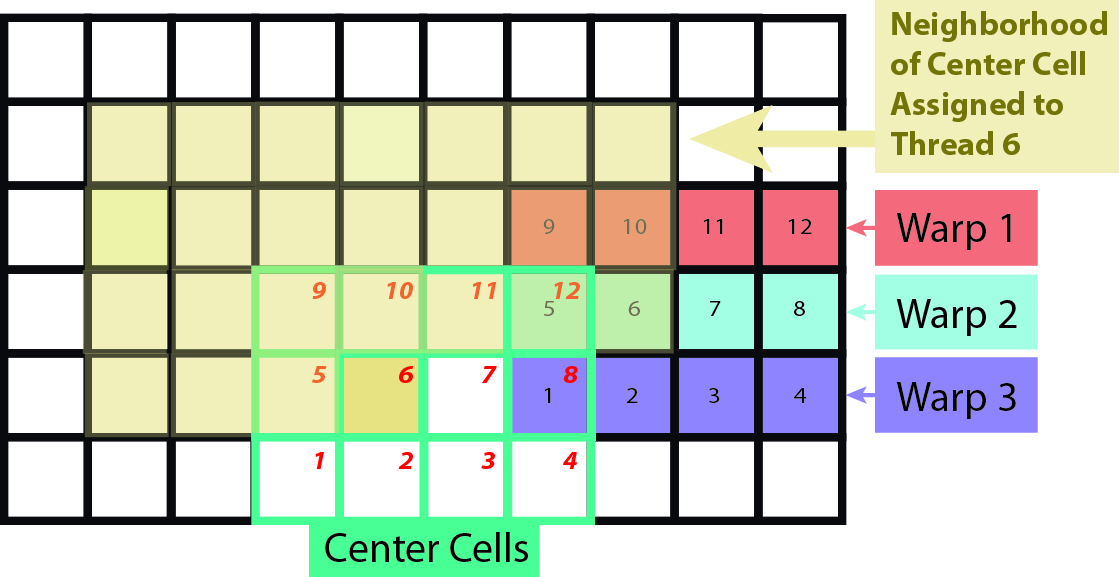
\includegraphics[width=1\columnwidth]{project22.jpg}

\end{figure}
CUDA's intra-warp implicit synchronization capability is the cornerstone
of our CUDA implementation of our pair-symmetric algorithm. Without
implicit synchronization, our pair-symmetric algorithm would render
useless for CUDA because it would require expensive synchronization
calls per Center-Neighbor Filter computation.

In CUDA, threads are organized into groups called warps. Each warp
executes one instruction at a time for its own group of threads. Essentially,
all the threads in a warp share the same program counter. Because
all threads in a warp share the same program counter and are therefore
driven by the same sequential instruction stream, all threads in a
warp are always in sync with each other without requiring explicit
synchronization calls. Therefore, synchronization between threads
in a warp is implicit.

To take full advantage of CUDA's implicit intra-warp synchronization
feature, divergent branching between threads in the same warp must
be avoided. This is so because all the threads in the same warp share
only one program counter. So, a divergent branch will cause some or
most of the threads to be idle as the program counter runs through
the branch and drives only those threads that meet the branch condition
to work. An example of a divergent branch can be a simple if-statement
such as: if (threadIdx.x < 5)\{...\} else\{...\}).

As it relates to stencil codes, divergent branching will commonly
occur in memory access patterns in which global memory operations
are not coalesced and shared memory operations are not free of memory
bank conflicts. For example, if eight threads were to read from eight
non-contiguous segments of global memory--such as that which is commonly
seen in strided access patterns like array{[}threadIdx.x {*} 2{]}--divergent
branching would occur because a warp of threads can only read from
one segment of memory per instructional transaction, and that segment's
word-length is hardware defined. In other words, a memory transaction
will be serialized unless all the threads in the warp to which the
transaction belongs are aligned consecutively and fit within a segment
of memory. Therefore, in order for all the threads of a warp to read/write
from global memory in a single transaction, the threads must correspond
read/write operations to aligned contiguous addresses within a segment
of memory. What this means in the implementation of stencil codes
is that warps should correspond to horizontal rows of pixels for an
i{*}jMax+j representation of a 2d image, for if threads in a warp
were to operate on pixels in a vertical order, there would be a separate
transaction for each thread in the warp, and if, for example, there
were two rows such that half of the threads were reading from memory
on each row, then there would be two transactions instead of one--i.e.,
inefficiency.

While intra-warp synchronization is guaranteed, the rate at which
warps stream through their sequence of instructions is unpredictable.
As a consequence, work must be arranged such that warps can work as
independent from each other as possible in order to minimize explicit
synchronization calls. This pooling of work is achieved by threads
reading from addresses incrementally along the horizontal axis, and
only making an explicit synchronization call per vertical shift to
the next row once the work requiring the warp's access to the instant
row of input data has completed. This design works because horizontal
shifts are implicitly synchronized as there is only one warp per row,
but a vertical shift without an explicit synchronization call will
result in a warp trespassing into the territory of another warp, thereby
causing race conditions as threads from two different warps will consequently
be prone to write to the same memory location.


\subsection{Shared Memory and Tile Processing}

CUDA features three types of memory with read/write capability suitable
for general-purpose computing on GPU: (1) global memory, which is
accessible by all threads in all thread blocks; (2) shared memory,
which is provided separately for each block of threads to share among
themselves; and (3) registers, which are separate and distinct for
each thread and of which each is only accessible by the thread to
which it belongs. Of these three types of memory, the slowest is global
memory, which unfortunately is where the host must first send the
input data before the GPU can begin its work. So, in order to see
any meaningful performance in CUDA, data stored in global memory must
be transferred to faster memory--i.e., shared memory, which is hundreds
of times faster. However, the trade-off is that the shared memory
size is much smaller than the global memory size, and this fact compels
a tile-based approach to stencil processing.

Our tile-based stencil processing approach is self-explanatory. Equal
sized partitions of the input data are processed, and then any remaining
data on and between the edge and the last partition that is closest
to (but not falling over) the edge boundary of the 2-dimensional data
representation is processed. With respect to the naive stencil code
algorithm, tile-based stencil processing is trivial and needs no further
explanation because simply partitioning the space and processing it
will suffice. However, for the pair-symmetric algorithm that we propose,
tile-based stencil processing requires adjustments in the order in
which tiles are processed in order to guarantee the exclusion of race
conditions. 

\begin{figure}
\caption{\label{fig:Tiling-for-Pair-Symmetric}Tiling for Pair-Symmetric Stencil
Processing:}


\includegraphics[width=1\columnwidth]{\string"stacked tiles\string".jpg}
\end{figure}


If processes were assigned to adjacent tiles, race conditions would
occur because the edge cells of the tiles, a by product of the Filter's
half-width, would overlap over each other, as illustrated in \ref{fig:Tiling-for-Pair-Symmetric}.
To get around this problem, simultaneously processed tiles can be
spaced apart in strides such that no two tiles being processed at
the same time intersect with one another. An example of such a technique
is illustrated in \ref{fig:An-iteration-of}(the tiles are flipped
sideways in this rendering).

\begin{figure}
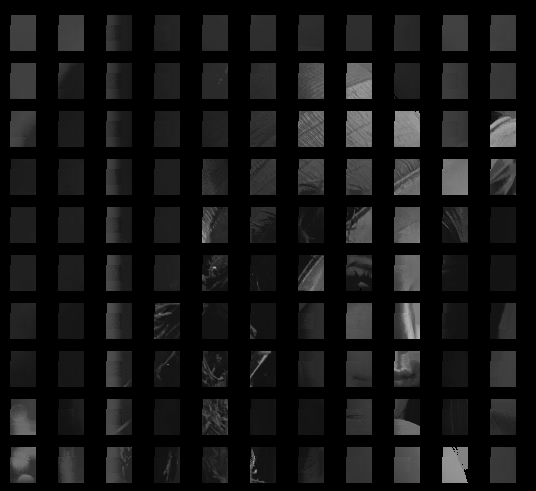
\includegraphics[width=1\columnwidth]{lenatiles}\caption{\label{fig:An-iteration-of}An iteration of processed tiles of Lena}
\end{figure}



\section{CPU-based Implementation Details}

\label{sec:optimizations} For regular numerical scientific computations
performance improvements in general can be achieved by parallelizing
the code either at low-level (micro-level or instruction level) or
at high-level (thread-level or task-based). For instance, $Intel$'s
Streaming SIMD Extension (SSE) is a technique to exploit micro-level
parallelism in x86 based processors using SIMD capabilities. SSE can
be ideal for tasks that involve repetitive computation such as the
3D heat equation defined in section \ref{sec:stencil} or any other
stencil kernel such as Jacobi iterations.

Researchers paid attention to the use of SSE instructions for scientific
applications almost a decade ago. Fundamental scientific kernels were
implemented to utilize SSE instructions which lead to some speedup.
For instance the matrix multiplication kernel was implemented in \cite{matrix-multi,MatrixMultiFloating}
for matrices with integers and floating point numbers. SSE instructions
have also been used for image or template matching algorithms such
as normalized cross correlation (``NCC'') \cite{NCCmatching}.

Task level parallelism can be achieved by utilizing multiple cores
in a system by using standard parallelization libraries such as Threaded
Building Block (``TBB''), OpenMP etc. Other traditional optimization
techniques such as loop unrolling, and prefetching etc. help to transform
the code into instruction level parallelism friendly code. Although,
the modern compilers usually try to improve the performance by automatically
vectorizing, unrolling loops, prefetching, and SIMDization, we were
still able to get significant performance improvements alongside compiler
optimizations.


\subsection{SIMD optimizations}

\label{sub:SIMD1} Modern day processors support SIMD optimizations
where the programmer can operate on multiple data elements in parallel
by storing the data into special purpose registers formerly known
as MMX\cite{MMX}, were introduced by Intel in 1996 to enhance multimedia
applications by exploiting their inherent parallelism. MMX has 8 64-bit
wide registers, which are consecutively named from MM0 to MM7. These
registers can hold 8 different bytes such as characters, or 4 words
such as short integers, 2 double words such as long integer, or single
precision float, or a single quad word such as double precision float.
A single MMX instruction can simultaneously process information stored
in these MMX registers, and therefore have the potential to provide
a speedup of up to 8 depending on the data type loaded into the registers.

Modern day CPUs use SSE that is an extension of MMX technology and
is fundamentally similar to MMX. It has 8 128-bit registers named
XMM0 through XMM7. SSE instructions can also operate in parallel on
data packed in these registers thus providing a theoretically maximum
speedup of 16. There are other extensions of SSE such as SSE2, SSE3,
and SSE4.2. Moreover, recent extension of SSE named Advanced Vector
Extensions (``AVX''), uses 256-bit data registers and thus a theoretical
peak speedup of 32 is possible.

Our implementation explores use of special purpose registers using
both assembly level programming and SSE intrinsics. The advantage
of using assembly language is that a programmer can have explicit
control of underlying hardware. However, programmer productivity is
affected and an in-depth knowledge of underlying hardware is essential.
Although, SSE intrinsics are wrappers for assembly language, it is
preferred to use SSE intrinsics due to ease of coding and also due
to efficient utilization of available assembly level instructions
without knowing the low level details of underlying architecture.
For instance, instructions that operate on aligned data usually perform
better than instructions that operate on unaligned data. A programmer,
working with intrinsics, can specify the intrinsic and the appropriate
instruction will automatically replace this intrinsic during compilation.
Moreover, there are some operations for which there are no assembly
instructions and hence in case of assembly level programming the code
size can grow to such an extent that readability gets compromised.


\subsection{Reduction Methods}

\label{sub:reduction} Sum by reduction is a technique to compute
sum of multiple elements usually stored in contiguous memory elements.
There are assembly instructions that can add horizontally packed,
single precision, floating point numbers. We used $haddps$ assembly
instruction that takes two (source and destination) 128 bit operands,
and adds the single precision floating point numbers stored in first
and second dword of destination and source operand and stores it in
first and third dword of the destination operand respectively. Similarly,
the third and fourth dword of destination and source operand are added
and stored in second and fourth dword of the destination operand respectively.
Both source and destination values must be stored in MMX registers.
The SSE intrinsic to perform horizontal add is $\_mm\_hadd\_ps$.
It takes two 128 bit operands, each of which is treated as four 32-bit
floating point elements. The result of this operation on operand X(X0,
X1, X2, X3) and Y(Y0, Y1, Y2, Y3) is (Y3 + Y2, Y1 + Y0, X3 + X2, X1
+ X0).


\section{Experimental Testbed}

\label{sec:expt}

\begin{table*}[t]
\begin{tabular}{|l|p{1.2cm}|p{0.8cm}|p{0.8cm}|p{0.8cm}|p{3.5cm}|l|p{2cm}|l|p{0.9cm}|}
\hline 
\textbf{Model}  & \textbf{Clock frequency}  & \textbf{cores per chip}  & \textbf{chips per node}  & \textbf{cores per node}  & \textbf{SIMD support}  & \textbf{Cache Memory}  & Compiler &  & \tabularnewline
\hline 
Intel Xeon E5410  & 2.33 GHz  & 4  & 2  & 8  & SSE, SSE2  & 12 MB  & icpc 11.1 &  & \tabularnewline
\hline 
Intel Xeon X7560  & 2.27 GHz  & 32  & 1  & 32  & SSE, SSE2  & 24 MB & icpc 11.1 &  & \tabularnewline
\hline 
Intel Core i7-870  & 2.93 GHz  & 4  & 1  & 4  & SSE, SSE2, SSE3, SSE4.2  & 8MB & icpc 12.0.2  &  & \tabularnewline
\hline 
AMD Opteron 2376  & 2.3 GHz  & 4  & 2  & 8  & SSE, SSE2  & 6MB  & icpc 11.1 &  & \tabularnewline
\hline 
AMD Opteron 8350  & 2.0 GHz  & 4  & 4  & 16  & SSE, SSE2  & 2MB  & icpc 11.1 &  & \tabularnewline
\hline 
AMD Phenom II X6 1045T  & 2.7 GHz  & 3  & 1  & 6  & SSE, SSE2, SSE4a  & 6MB  & icpc 12.0.2  &  & \tabularnewline
\hline 
\end{tabular}\caption{Architectural details of multicore chips employed for experiments}


\label{tab:archs} 
\end{table*}


In order to evaluate our implementation we have tried it on a range
of multicore chips. Table \ref{tab:archs} summarizes architectural
details of systems we used during our experiments. 


\subsection{Hardware}

\label{subsec:hw} 


\subsubsection{Intel Xeon}

\label{ss:xeon} We have used two different Xeon chips, E5410 (Harpertown)
and X7560 (Nehalem EX). Harpertown is a dual-socket, dual-processor
relatively old system with a clock frequency of 2.33 GHz. Our computing
node has two Harpertown chips with total number of cores being eight.
It does not have Intel's hyperthreading (HT) technology which means
the maximum number of threads is equal to the number of cores available.
Intel Nehalem EX is considerably newer chip having eight-cores per
processor with each core having clock frequency of 2.27 GHz. We had
access to a Linux cluster from Intel's Manycore Testing Lab (MTL)
containing four sockets of Nehalem EX chips thereby making 32 cores
available to experiment with. The processors are connected to each
other via Intel QPI (Quickpath interconnect) links that can transfer
data at 6.4 GT/s. Both of these machines support 64 bit instructions. 


\subsubsection{AMD Opteron}

\label{ss:opteron} AMD Opteron 2376 (Shanghai) chip has private L1
and L2 caches of size 128KB (64 D + 64 I) and 512KB respectively per
core along with a 6MB cache shared among all of the cores. It has
a clock frequency of 2.30 GHz and it is a quad-core architecture.
Our compute node has two of Shanghai chips making it a total of eight
cores to be used for experiments. AMD Opteron 8350 (Barcelona) is
similar to Shanghai in many aspects but it has a clock frequency of
2.0 GHz and the shared cache is only 2MB. Our compute node contains
4 of Barcelona chips and thus we are able to run 16 threads on this
node. 


\subsubsection{Intel Core i7}

\label{ss:corei7}Intel Core i7 - 870 code named Lynnfield supports
SSE 4.2 and has AVX technology. The clock frequency is an impressive
2.93 GHz and it can operate at a maximum of 3.6 GHz thanks to Intel's
power boost technology. Lynnfield supports hyperthreading which lets
an application to execute 8 threads. It contains 2 memory channels
that provide a theoretical maximum memory bandwidth of 21 GB/s. 


\subsubsection{AMD Phenom II}

\label{ss:phenom} AMD Phenom is a six core processor with each core
capable of operating at 2.7 GHz. If only three cores are in operation
it can run at a maximum of 3.2 GHz. It boasts 128 KB (64 D + 64 I)
L1 cache, and 512 KB L2 cache per core in addition to a 6MB L3 cache
shared among all six cores. The cache latencies are 3, 13, and 47
clock cycles for L1, L2, and L3 caches respectively. The cache line
size is 64 bytes, L1 caches are 2 way set associative, L2 caches are
16-way set associative and L3 cache is 48-way set associative.


\subsection{Software Framework}

\label{subsec:sw} Our implementation is written in $C++$ and uses
OpenMP for parallelization. To enrich supported image formats by our
implementation we use $CImg$ library. Intel Vtunes Amplifier XE was
used to find out hotspots in our code. 


\subsubsection{Algorithms}

We have implemented a number of variations of bilateral filtering
kernel, results of which are reported in section \ref{sec:results}.
These algorithms are labeled as follows: 
\begin{itemize}
\item $BL\_Naive$ is the sequential version of the code, as described by
\cite{Tomasi1998}. 
\item $BL\_Naive\_No\_Exp$ is similar to sequential version in all aspects,
except the fact the most time consuming $exp$ instruction, discussed
after this list of algorithms, is commented out. 
\item $BL\_Tiles$ is the version that employs data blocking while processing
the input image. 
\item $BL\_Tiles\_No\_Exp$ is to $BL\_Tiles$ what $BL\_Naive\_No\_Exp$
is to $BL\_Naive$. 
\item $BL\_Assembly$ is the version of bilateral filtering implemented
using assembly level code. 
\item $BL\_A\_Reduction$ is the version of bilateral filtering that uses
assembly language as well as reduction optimizations. 
\item $BL\_Intrinsic$ version uses SSE intrinsics instead of assembly language. 
\item $BL\_I\_Reduction$ is the extended version of $BL\_Intrinsic$ that
uses the intrinsics that can compute sum of two 128 bit operands in
parallel. 
\end{itemize}
$BL\_Naive$ has a redundant calculation inside the innermost loop
which has been moved out of loop for all other versions. The original
instruction involving this calculation looks like\\
 $gaussian\_ph=exp(-(pd)/(2*(sigma\_ph*sigma\_ph)));$\\
 After moving the redundant calculation out of the loop the same instruction
becomes\\
 $gaussian\_ph=exp(pd*pre\_calc\_sigma\_sq));$\\



\subsubsection{Input Image}

In order to analyze the behavior of our kernel with varying image
sizes, we have executed our kernel with two different images. One
that fits into cache easily and the other that does not fit into cache
but fits into main memory. Both of the images were converted to single
spectrum images represented by single precision numbers for each pixel.
The smaller image was 512 pixels wide and 512 pixels high, thus requiring
1MB memory to store it. As shown in table \ref{tab:archs} all of
the systems have cache memories bigger than 1 MB. The second image
was 3000 pixels wide and 3000 pixels high and hence requires little
more than 34 MB of memory to store it. None of the cache memories
were such big to store this image entirely.


\section{Performance Results}

\label{sec:results}

\begin{figure*}[t!]
 

\begin{centering}
\subfigure[Small Image]{ 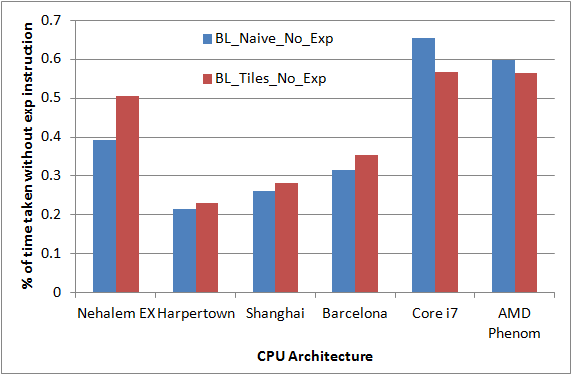
\includegraphics[width=3.2in,height=2in]{noexpsmall}
\label{fig:smallnoexp} } \subfigure[Large Image]{ 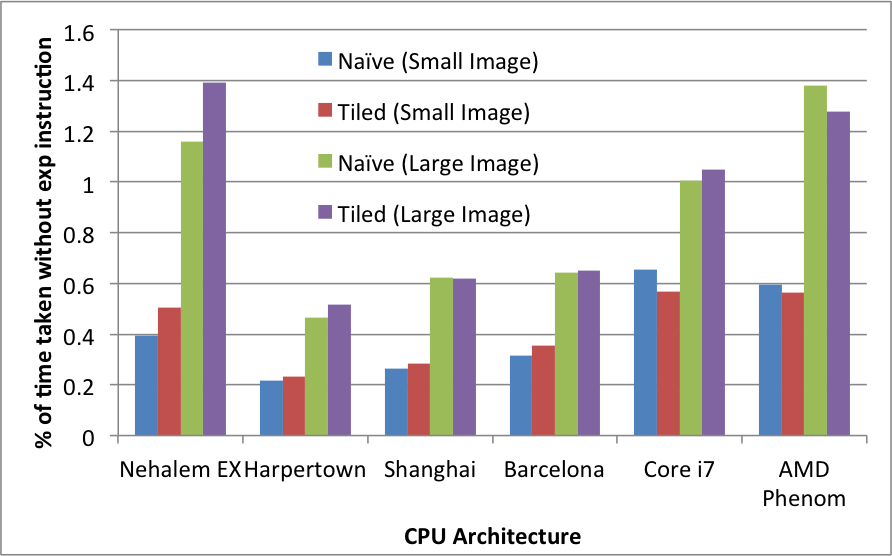
\includegraphics[width=3.2in,height=2in]{noexplarge}
\label{fig:largenoexp} } 
\par\end{centering}

\caption{Percentage of time taken by sequential kernel when run without $exp$
instruction, $filter$ $radius$=10.}


\label{fig:noexp} 
\end{figure*}


For all of our experiments the filter radius was kept at 10, subsequently
making the Window of size 21 x 21. The spatial spread and the photometric
spread were also set to 10. The optimization flag O3 was used for
all experiments in addition to SSE2 for SIMDization. For Core i7 chip
compiler flag SSE4.2 was used instead of SSE2. We do not use hyperthreading
which means there are no more than one thread per core. 
\begin{figure*}[t!]
 

\begin{centering}
\subfigure[Nehalem-EX Xeon X7650]{ \includegraphics[width=3.2in,height=2.3in]{nehalem}
\label{fig:Nehalem} } \subfigure[Harpertown Xeon E5410]{ 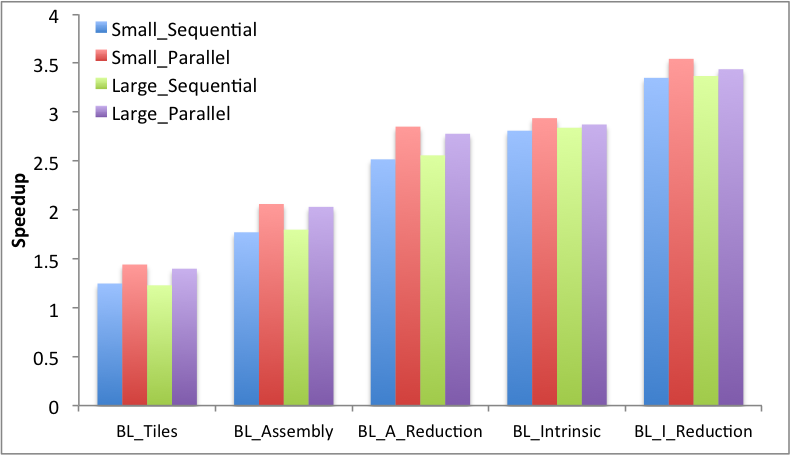
\includegraphics[width=3.2in,height=2.3in]{harpertown}
\label{fig:harpertown} } \subfigure[Core i7 - 870]{ 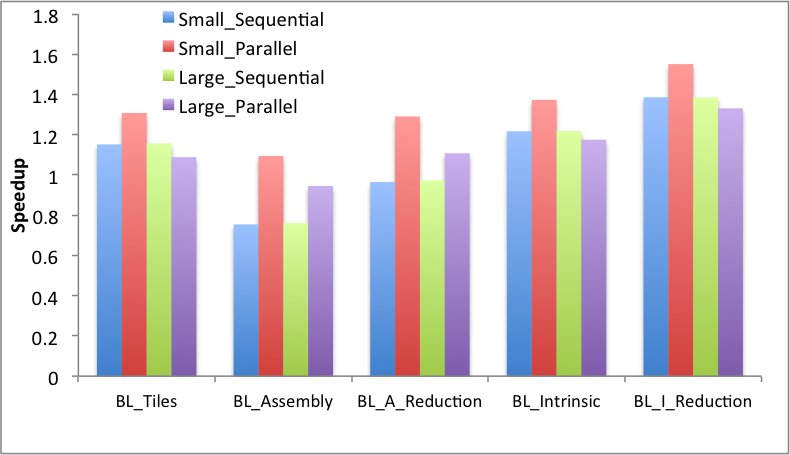
\includegraphics[width=3.2in,height=2.3in]{corei7}
\label{fig:corei7} } 
\par\end{centering}

\caption{Performance of different algorithms for bilateral filtering kernel
on Intel chips for both small image and large image. Sequential version
(Small\_Sequential, Large\_Sequential) does not use OpenMP while Parallel
version (Small\_Parallel, Large\_Parallel) uses all available cores.
The comparison is with BL\_Naive version, auto optimized by compiler
with -O3 and -xSSE2 flags. }


\label{fig:comparisonIntel} 
\end{figure*}


\begin{figure*}
\begin{centering}
\subfigure[Barcelona AMD Opteron 8350]{ 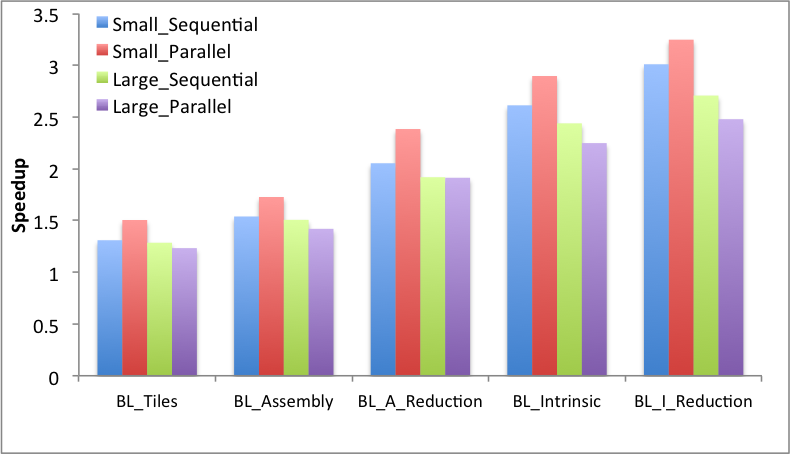
\includegraphics[width=3.2in,height=2.3in]{barcelona}
\label{fig:barcelona} } \subfigure[Shanghai AMD Opteron 2376]{
\includegraphics[width=3.2in,height=2.3in]{shanghai} \label{fig:Shanghai}
} \subfigure[AMD Phenom II 1045T]{ 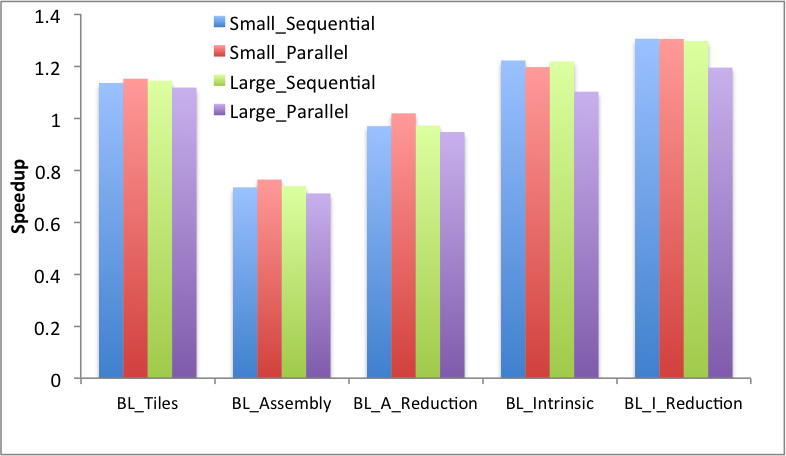
\includegraphics[width=3.2in,height=2.3in]{phenom}
\label{fig:Phenom} } 
\par\end{centering}

\caption{Performance of different algorithms for bilateral filtering kernel
on AMD chips for both smaller image and larger image. Sequential version
(Small\_Sequential, Large\_Sequential) does not use OpenMP while Parallel
version (Small\_Parallel, Large\_Parallel) uses all available cores.
The comparison is with BL\_Naive version, auto optimized by compiler
with -O3 and -xSSE2 flags.}


\label{fig:comparisonAMD} 
\end{figure*}


\begin{figure*}[t!]
 

\begin{centering}
\subfigure[Harpertown Xeon E5410]{ 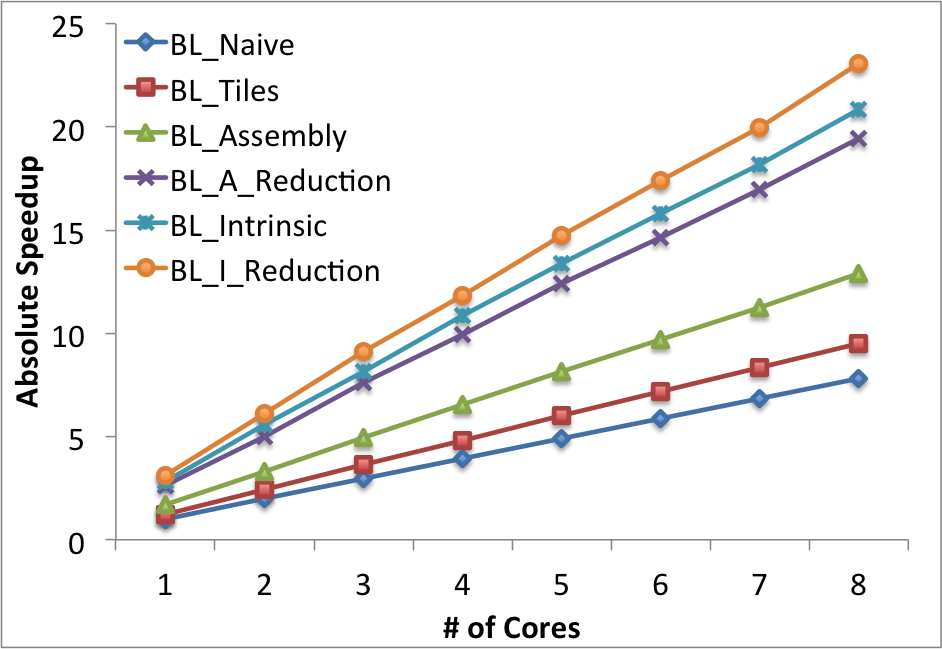
\includegraphics[width=3.2in,height=2.5in]{harpertownfinal}
\label{fig:harpertownFinal} } \subfigure[Core i7 - 870]{ \includegraphics[width=3.2in,height=2.5in]{corei7final}
\label{fig:corei7Final} } \subfigure[Nehalem-EX Xeon X7650]{ \includegraphics[width=4.2in,height=3.5in]{nehalemfinal}
\label{fig:NehalemFinal} } 
\par\end{centering}

\caption{Comparison of combined speedup due to SIMDization and OpenMP parallelization
on Intel chips for different algorithms}


\label{fig:comparisonFinalIntel} 
\end{figure*}


\begin{figure*}
\begin{centering}
\subfigure[Barcelona AMD Opteron 8350]{ 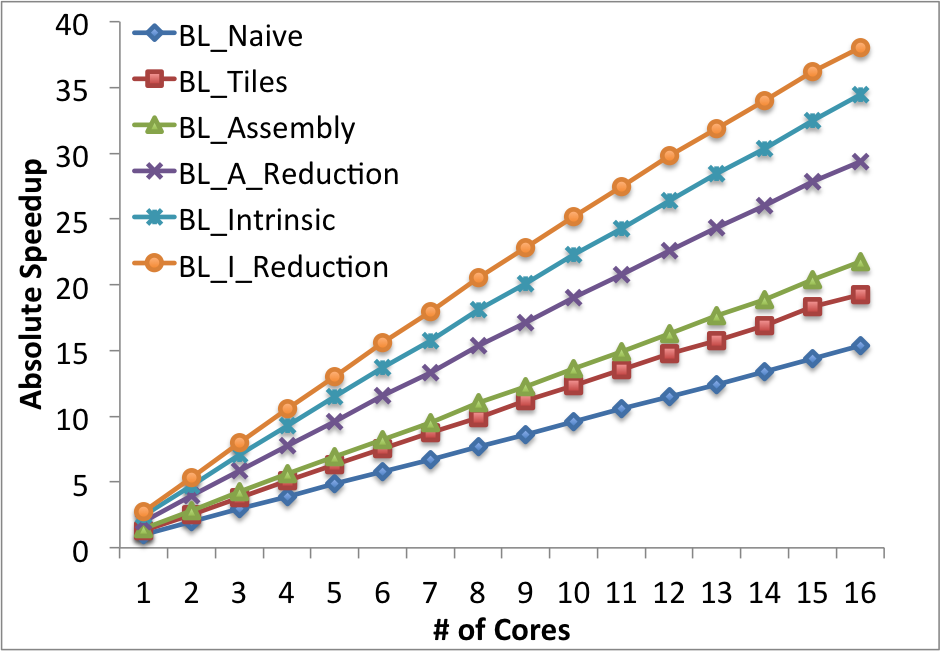
\includegraphics[width=3.2in,height=2.5in]{barcelonafinal}
\label{fig:barcelonaFinal} } \subfigure[Shanghai AMD Opteron 2376]{
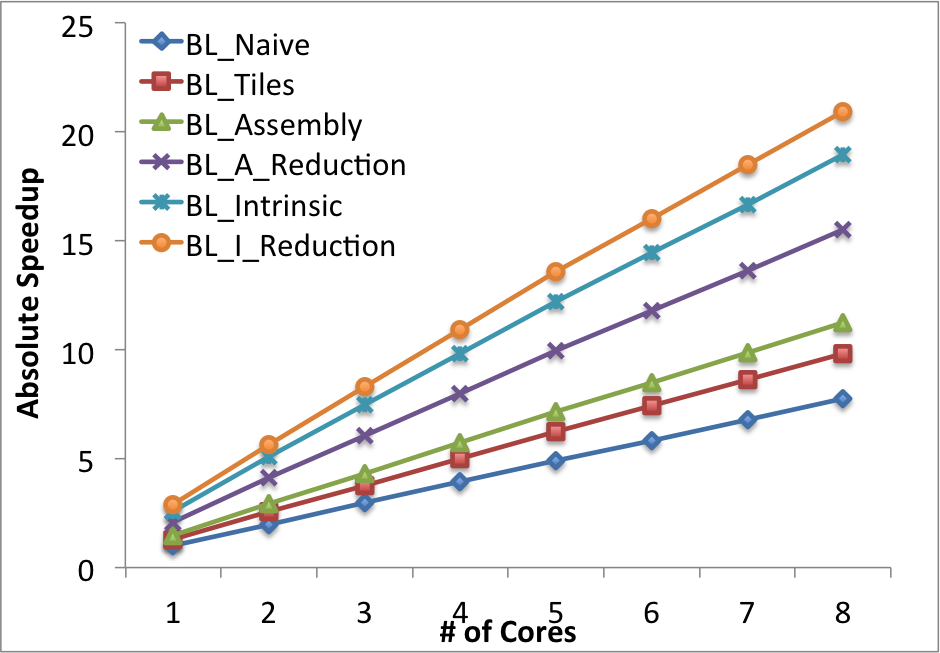
\includegraphics[width=3.2in,height=2.5in]{shanghaifinal} \label{fig:ShanghaiFinal}
} \subfigure[AMD Phenom II 1045T]{ 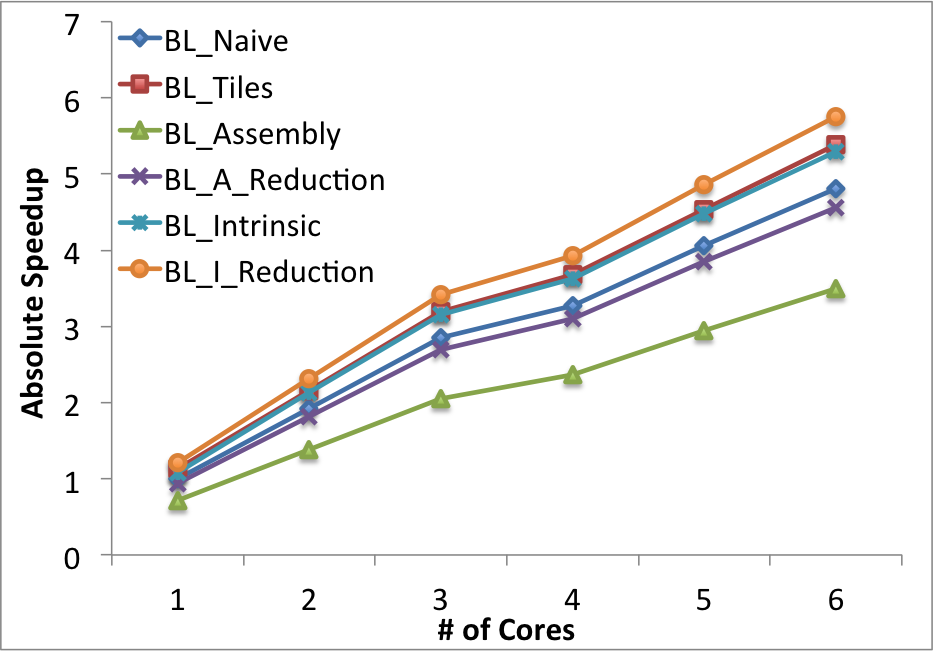
\includegraphics[width=3.2in,height=2.5in]{phenomfinal}
\label{fig:PhenomFinal} } 
\par\end{centering}

\caption{Comparison of combined speedup due to SIMDization and OpenMP parallelization
on AMD chips for different algorithms.}


\label{fig:comparisonFinalAMD} 
\end{figure*}


Running the hotspot analysis it was realized that the most time consuming
instruction was the instruction involving computation of exponential
function for the photometric kernel. Figure~\ref{fig:noexp} shows
the percentage of time taken by $BL\_Naive\_No\_Exp$ and $BL\_Tiles\_No\_Exp$
on different platforms for both smaller image (figure~\ref{fig:smallnoexp})
and the larger image (figure~\ref{fig:largenoexp}). It can be seen
that after taking the $exp$ instruction out of the computation the
total sequential execution time is consistently less than 2\% of the
execution time with $exp$ instruction in place. For the smaller image
it is strictly less that 1\% of the time with $exp$ instruction in
place. To be precise it is 1.39\% maximum on Intel Nehalem for the
larger image and 0.65\% for the smaller image on Core i7 processor.
The lower memory transfer time for smaller image is due to the fact
that the smaller image sits into the cache memory entirely and hence
there are no repeated data transfers between processor and main memory.

Since the $exp$ instruction does not involve transfer of data from
main memory, it is logical to deduce from this experiment that memory
reuse and memory access pattern related optimizations are not of much
help to speed up bilateral filtering kernel. What Amdahl's law claims
for inherently sequential portion of the code can be applied here.
\\
 \textit{The total speedup achieved by optimizations that deal with
memory management is limited by the amount of time spent in memory
transfers}. Therefore, in this case traditional optimizations such
as tiling/blocking, cache efficient initializations, prefetching,
and other NUMA optimizations can only result in a speed up of at most
2\%.

Figure~\ref{fig:comparisonIntel} compares different algorithms on
different Intel chips. In this experiment we are comparing the speedup
achieved by the respective algorithm compared to BL\_Naive algorithm.
It is important to note that these results are for micro level parallelism
(use of 128 bit special purpose registers) only and do not consider
speedup due to high level (OpenMP) parallelization. We have used parallel
version, that utilizes all available cores on that chip, only to show
that the speedup is still bounded by the theoretical peak speedup
which happens to be four here since we work with 32bit floating point
numbers. Interestingly, since we use compiler optimization flags such
as -O3 and -xSSE2 there is automated vectorization taking place in
all the algorithms. However, our hand coded vectorization is superior
in most of the cases.

The speedup shown by BL\_Tiles is mostly due to the computation reduction
as discussed in section \ref{subsec:sw} because we do not use special
purpose registers in this algorithm. It can be seen from figure~\ref{fig:comparisonIntel}
that the parallelism due to SIMDization is limited by four which is
the theoretical maximum possible speedup due to SSE registers as discussed
in section \ref{sub:SIMD1}.

As seen in figure~\ref{fig:Nehalem} the maximum speedup achieved
on Nehalem architecture only using SSE optimization is 2.29x for the
smaller image and 1.33x for the larger image. Smaller image generally
performs better because the time to copy data to SSE registers is
less as the entire image is always available in the cache memory.
The BL\_Naive algorithm outperforms our assembly level implementations
but it is slower than our intrinsic based implementations in all cases.
The reason for this is that the auto SIMDization by compiler is more
efficient than our implementation for Nehalem architecture. Intel
Harpertown, which is a relatively older chip, shows an impressive
speedup of 3.54x (figure~\ref{fig:harpertown}) even though compiler
optimizations are still in place. Another interesting observation
is the results on Intel Core i7 architecture (figure~\ref{fig:corei7}).
The reason for this behavior is the newer compiler. These experiments
were run with $SSE4.2$ compiler flag and hence the compiler is able
to exploit SIMDization automatically thus making it difficult to surpass
it using assembly level coding. However, our algorithms that use SSE
intrinsics and reduction, i.e. BL\_A\_Reduction, BL\_Intrinsic, and
BL\_I\_Reduction are able to provide greater speedups than those achieved
by compiler optimizations as shown in figures~\ref{fig:comparisonIntel},
and \ref{fig:comparisonAMD}.

Figure~\ref{fig:comparisonAMD} shows the same comparison across
AMD chips. The results are in tune with those for Intel platform.
As shown in figure~\ref{fig:barcelona} for Barcelona, which is a
relatively older chip, the maximum speedup is 3.24x for BL\_I\_Reduction
algorithm. Similarly, for AMD Shanghai, as shown in figure~\ref{fig:Shanghai},
the maximum speedup achieved by exploiting SIMDization is 3.02x for
BL\_I\_Reduction algorithm. The case of AMD Phenom is shown in figure~\ref{fig:Phenom}.
It can be seen that similar to Intel Core i7 and Intel Nehalem architecture
the newer compiler by Intel affects the performance here too. The
auto tuning applied by the compiler outperforms the manual tuning
in case of BL\_Assembly and BL\_A\_Reduction. However, BL\_Intrinsic
and BL\_I\_Reduction are still able to outperform compiler optimizations.
The maximum speedup achieved in this case is 1.30x.

Figure~\ref{fig:comparisonFinalIntel} shows the speedup with increasing
number of OpenMP threads for the larger image. It is interesting to
see how speedup due to OpenMP multiplies with the speedup due to SSE
optimizations to exhibit super linear performance. Although the input
images are not very large to provide enough grain to a machine with
32 cores, the kernel still scales well. For other architectures the
kernel demonstrates super-linear behavior.

Figure~\ref{fig:harpertownFinal} shows the performance of bilateral
filtering kernel on Intel Harpertown. This machine has 8 cores and
the maximum combined speedup achieved is 20.91x. The speedup achieved
only using only SSE optimization was 2.69x and the speedup achieved
by BL\_Naive algorithm using 8 cores is 7.73x.

Intel Nehalem chip with 32 cores does not show a super-linear speedup
as shown in figure~\ref{fig:NehalemFinal}. However, the reason behind
this is the lack of enough parallelism that can be afforded by the
kernel for this image. Both optimizations still multiply their individual
speedup to result in the combined speedup. The total combined speedup
is 26.46x using 32 cores, the speedup only due to SSE was 1.12x and
the speedup for BL\_Naive is 23.47x.

Intel Core i7 chip (figure~\ref{fig:corei7Final}) demonstrates the
similar behavior too. The final speedup of 4.63x, using 4 cores, is
a result of speedup due to SSE which is 1.33x and speedup due to OpenMP
which is 3.48x. Figure~\ref{fig:comparisonFinalAMD} shows a similar
comparison over various AMD chips. Figure~\ref{fig:barcelonaFinal}
shows the speedup for Barcelona chip. This chip has 16 cores with
a combined maximum speedup being 38.03x. The speedup achieved using
SSE optimizations was 2.48x and the speedup for BL\_Naive was 15.34x
and thus these both realize a speedup of 38.03x using 16 cores.

AMD Shanghai similarly shows an impressive speedup of 20.92x (figure~\ref{fig:ShanghaiFinal}).
The interesting case is with AMD Phenom as shown in figure~\ref{fig:PhenomFinal}.
The speedup drops a little as number of cores increases beyond three.
The reason behind this is the turbo core technology as discussed in
section (\ref{ss:phenom}). When there are a maximum of three cores
being used the clock frequency scales up to 3.6 GHz but as soon as
more threads are created the clock frequency steps down to 2.7 GHz. 


\section{Conclusion and future work}

\label{sec:conclusion} Modern day scientific applications demand
higher computational capabilities than before and performance gains
are no longer driven by clock speed. Chip manufacturers are trying
to meet this demand by adding multiple cores on a chip equipped with
multiple levels of cache hierarchy and enhanced SIMD extensions. In
this paper we have tried to optimize bilateral filtering kernel using
both high level and low level parallelism. Our interest is to develop
an efficient parallelization method for modern multicore architectures
that can be applied to any spatially invariant and inseparable filter
kernel and potentially to any compute-intensive regular numeric application.
We have also documented why traditional optimization methods for multicores
are not as effective for bilateral filtering kernel compared to memory
intensive kernels. It can be seen from figure~\ref{fig:comparisonIntel},
and figure~\ref{fig:comparisonAMD} that a stencil kernel could be
optimized by using SSE intrinsics even though the compiler optimizations
are in place. Moreover, the reduction methods can provide a decent
speedup where applicable. These findings will guide the auto optimizers
and auto tuners to include SSE intrinsics as an essential optimization
approach.

\begin{figure}[h!]
\includegraphics[width=3.2in]{Gpu} \caption{Execution time of bilateral filtering on GPU with increasing number
of threads per block for larger image, $filter$ $radius$=10, $spatial$
$spread$=10, $photometric$ $spread$=10}


\label{fig:gpu} 
\end{figure}


We have also ported bilateral filtering to GPU. As shown in figure~\ref{fig:gpu}
we are able to use up to 90,000 threads per block with total number
of blocks being 10. Each thread is processing one pixel of the larger
image which has a height of 3000 pixels and width of 3000 pixels too.
The results are promising and we are exploring the software controlled
memory hierarchy and registers in an efficient ways as future work
of this research.

\bibliographystyle{IEEEtran}
\bibliography{paper}
 
\end{document}
